\documentclass[11pt, a4paper]{article}

\usepackage[ngerman]{babel}
\usepackage{hyperref}
\usepackage{graphicx} 
\usepackage[utf8]{inputenc}
\usepackage{fancyhdr}
\usepackage{changepage}
\usepackage[onehalfspacing]{setspace}
\usepackage{ragged2e}
\usepackage{ amssymb, amsmath, amsthm, dsfont }
\usepackage[width = 18cm, top = 2.5cm, bottom = 3cm]{geometry}
\usepackage{extarrows}
\usepackage{listings,color}
\usepackage[usenames,dvipsnames,svgnames,table]{xcolor}
% --------- Variabel, auf jedem Blatt ändern!
\newcommand{\blattnummer}{8}
\newcommand{\datum}{21. Juni 2017}
	% Punktezahlen & Summe
\newcommand{\p}{8}
\newcommand{\pp}{7}
\newcommand{\ppp}{5}
\newcommand{\pppp}{}
\newcommand{\sump}{20}
% --------- Macros

\newcommand{\myTitleString} {}
\newcommand{\myAuthorString} {}
\newcommand{\mySubTitleString} {}
\newcommand{\myDateString} {}

\newcommand{\myTitle}[1] {\renewcommand {\myTitleString}{#1}}
\newcommand{\mySubTitle}[1] {\renewcommand {\mySubTitleString}{#1}}
\newcommand{\myAuthor}[1] {\renewcommand{\myAuthorString}		{#1}}
\newcommand{\myDate}[1] {\renewcommand{\myDateString}{#1}}

\makeatletter
\newcommand*{\centerfloat}{%
  \parindent \z@
  \leftskip \z@ \@plus 1fil \@minus \textwidth
  \rightskip\leftskip
  \parfillskip \z@skip}
\makeatother

\newcommand{\makeMyTitle}
{
\pagestyle{fancy}
\fancyhead[L]
{
\begin{tabular}{l}
\myTitleString
\\ \mySubTitleString 
\\ \myDateString
\end{tabular}
} 			
\fancyhead[C]{}
\fancyhead[R]{\myAuthorString}
\fancyfoot[C]{\thepage}
}

\setlength{\headheight}{45pt}

\makeatletter
\renewcommand*\env@matrix[1][*\c@MaxMatrixCols c]{%
  \hskip -\arraycolsep
  \let\@ifnextchar\new@ifnextchar
  \array{#1}}
\makeatother

    % args: Aufgabennummer, erreichbare Punkte
\newcommand{\aufgabe}[2] {\section*{Aufgabe \blattnummer.#1 (Punkte:\qquad/#2)}}
\newcommand{\aufgabenteil}[1] {\textbf{(#1)}}
% ---------
%\setlength{\parindent}{0pt}
\begin{document}

\myTitle{\textsc{Datenbanken und Informationssysteme}}
\mySubTitle{Übung \blattnummer}
\myDate{\datum}
\myAuthor
{
\begin{tabular}{l l}
359109, &Michelle Milde\\
356148, &Philipp Hochmann\\
356092, &Daniel Schleiz
\end{tabular}
}
\makeMyTitle

\hfill
\begin{tabular}{|c|c|c|c|}\hline
   1 & 2 & 3 & $\sum$\\\hline
  	 \qquad/\p & \qquad/\pp & \qquad/\ppp & \qquad/\sump\\\hline % abhängig vom Übungsblatt
 \end{tabular}
\hfill Korrigiert am:\underline{\hspace{3cm}}
\hfill
\vspace*{30pt}


\aufgabe{1}{\p}
\aufgabenteil{a}\\
	\lstset{
    language=xml,
    tabsize=3,
    %frame=lines,
    caption=Bundestagswahl.xsd,
    label=code:sample,
    frame=shadowbox,
    rulesepcolor=\color{gray},
    xleftmargin=20pt,
    framexleftmargin=15pt,
    keywordstyle=\color{blue}\bf,
    commentstyle=\color{OliveGreen},
    stringstyle=\color{red},
    numbers=left,
    numberstyle=\tiny,
    numbersep=5pt,
    breaklines=true,
    showstringspaces=false,
    basicstyle=\footnotesize,
    emph={food,name,price},emphstyle={\color{OliveGreen}}}
    \lstinputlisting{Bundestagswahl.xsd}
\aufgabenteil{b}\\
    \lstset{
    language=xml,
    tabsize=3,
    %frame=lines,
    caption=Bundestagswahl-daten.xml,
    label=code:sample,
    frame=shadowbox,
    rulesepcolor=\color{gray},
    xleftmargin=20pt,
    framexleftmargin=15pt,
    keywordstyle=\color{blue}\bf,
    commentstyle=\color{OliveGreen},
    stringstyle=\color{red},
    numbers=left,
    numberstyle=\tiny,
    numbersep=5pt,
    breaklines=true,
    showstringspaces=false,
    basicstyle=\footnotesize,
    emph={Bundestagswahl,Wahlkreis,Datum,Bezeichnung,Erststimmen,Kandidatenstimmen,Kandidat,Name,Beruf,Telefonnummer,Anzahl,Ungueltig,Zweitstimmen,Parteistimmen,Partei},emphstyle={\color{magenta}}}
    \lstinputlisting{Bundestagswahl-daten.xml}


\aufgabe{2}{\pp}
\aufgabenteil{a}
\begin{adjustwidth}{20pt}{20pt}

\end{adjustwidth}
\aufgabenteil{b}
\begin{adjustwidth}{20pt}{20pt}

\end{adjustwidth}
\aufgabenteil{c}
\begin{adjustwidth}{20pt}{20pt}

\end{adjustwidth}
\aufgabenteil{d}
\begin{adjustwidth}{20pt}{20pt}

\end{adjustwidth}
\aufgabenteil{e}
\begin{adjustwidth}{20pt}{20pt}

\end{adjustwidth}



\aufgabe{3}{\ppp}
\aufgabenteil{a}
\begin{figure}[h]
\centerfloat
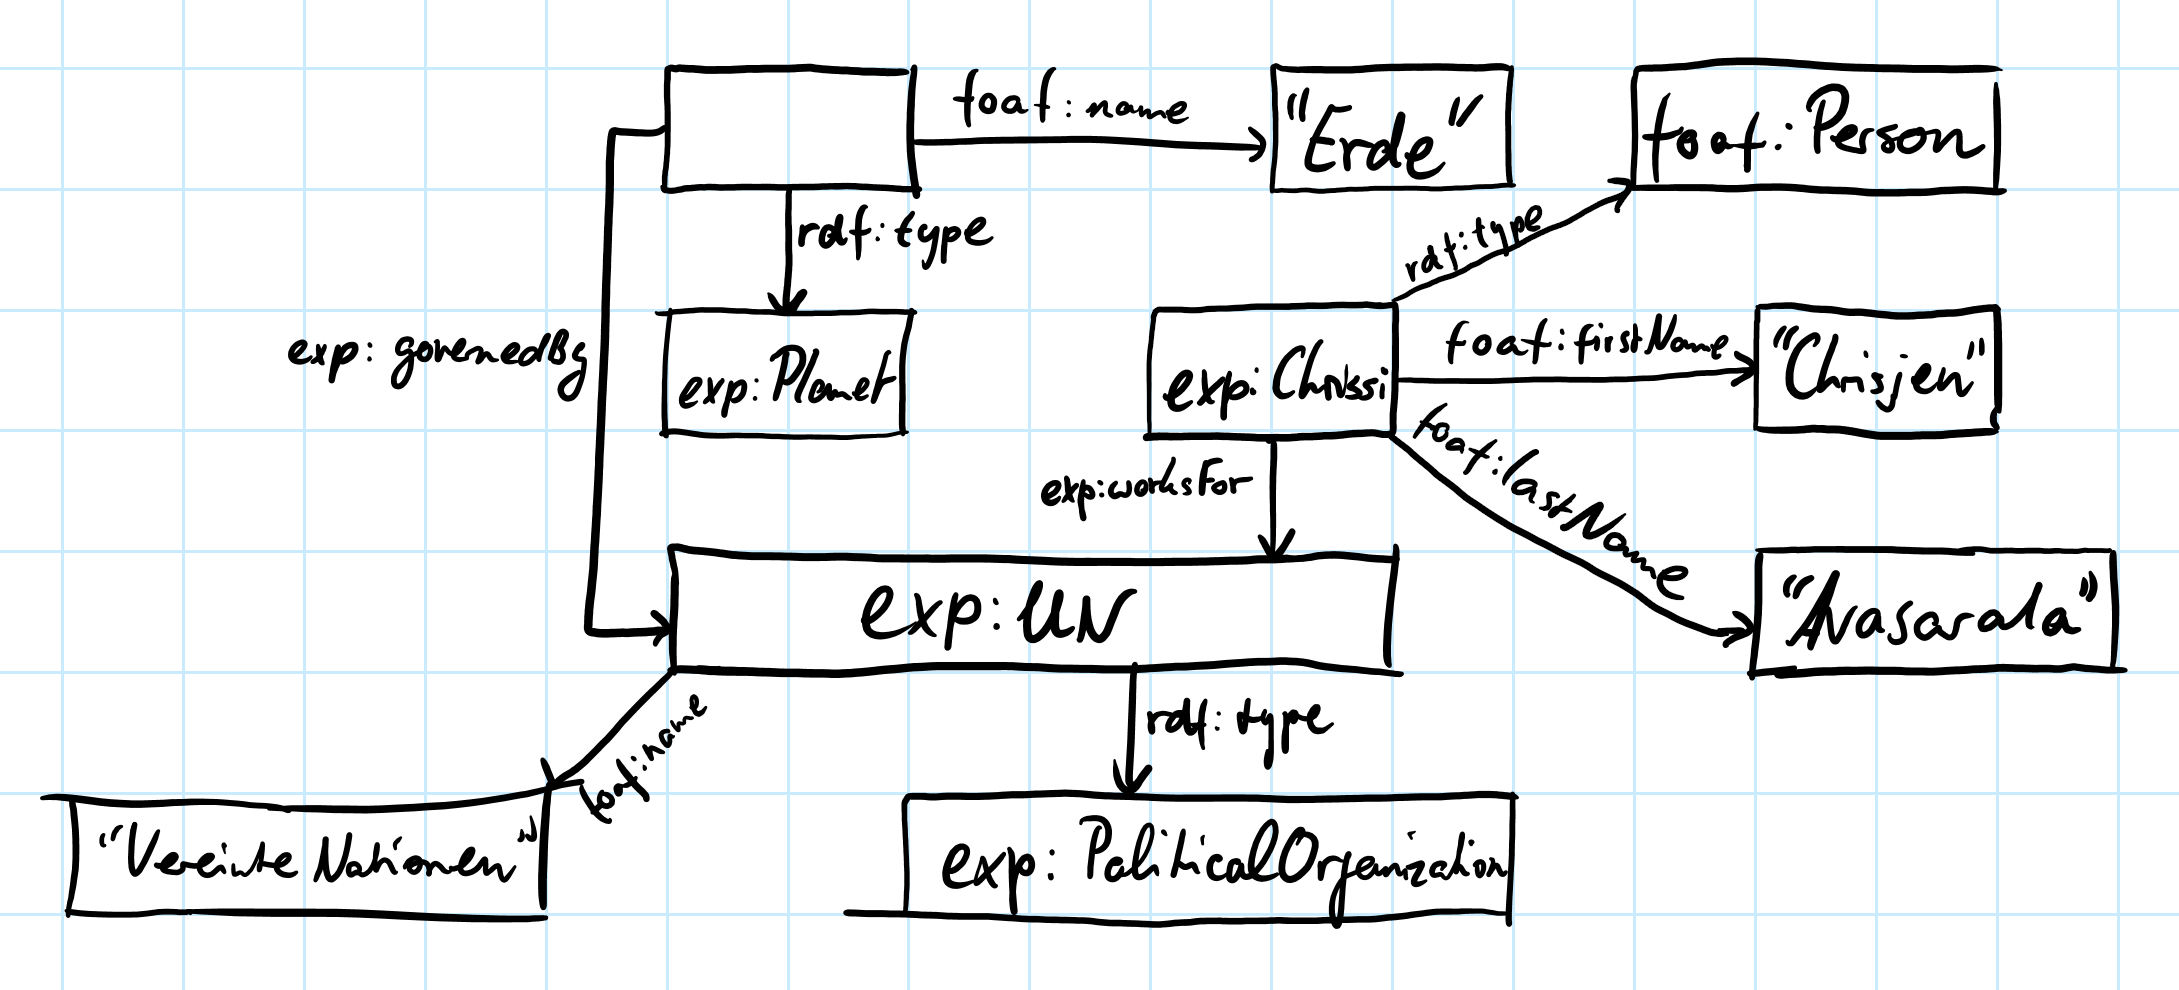
\includegraphics[page=1,scale=0.5]{u08-3-a.png}
\end{figure}
\newpage
\aufgabenteil{b}
\begin{adjustwidth}{20pt}{20pt}
$@$prefix rdf: $<$\url{http://www.w3.org/1999/02/22-rdf-syntax-ns\#}$>$ .\\
$@$prefix foaf: $<$\url{http://xmlns.com/foaf/0.1/}$>$ .\\
$@$prefix exp: $<$\url{http://example.org/the-expanse/}$>$ .\\
\\ \ \\
\shorthandon{"}
$<\_>$ foaf:name ``Erde'' .\\
$<\_>$ rdf:type exp:Planet .\\
$<\_>$ exp:governedBy exp:UN .\\
exp:Chrissi foaf:firstName ``Chrisjen'' .\\
exp:Chrissi rdf:type foaf.person .\\
exp:Chrissi foaf:lastName ``Avasarala'' .\\
exp:Chrissi exp:worksFor exp:UN .\\
exp:UN foaf:name ``Vereinte Nationen'' .\\
exp:UN rdf:type exp:PoliticalOrganization .\\
\shorthandoff{"}
\end{adjustwidth}

% --------
\end{document}
